\section{Distributed storage services}\label{sec:distributedStorage}
The idea of accessing files via the network can be traced back to the early days
of the internet. However, the first widely used implementation of a networked
filesystem was developed by SUN Microsystems\cite{nfs1986}. Their implementation
is widely reffered to as the networked filesystem(NFS). Their implementation
provided users with the ability to mount a filesystem present on a remote
machine. However, this system did not provide any distribution transparency as
the users had to be aware of where and how each file is stored on remote
machines. 

\medskip
The first widely used implementation of a distributed filesystem is considered
to be the Hadoop Distributed Filesystem (HDFS)\cite{shvachko2010hadoop}. This
implementation provided distribution transparency and consistency gaurantees on
various operations on the files stored in HDFS. This implemnetation was inspired
by the Google Filesystem\cite{ghemawat2003google} which was developed by Google
in 2003 almost seven years before HDFS.

\medskip
Although filesystems like HDFS were widely used, filesystems like AWS
S3\cite{awsS3} provided an additional feature of being multi-tenant. In other
words, with filesystems like AWS S3, a user could reap the benefits of a
distributed filesystem without having to manage or pay for an entire cluster.
The cost of managing, scaling, and maintaining the distributed cluster was
delegated to cloud providers like AWS. Now, users could pay for the amount of
data that they store, and the number of requests that they make to their data.
This has enabled the usage of such distributed filesystems in applications like
video streaming, database storage\cite{snowflake}, web content 
delivery, and backup storage.

\begin{figure}[ht]
    \centering
    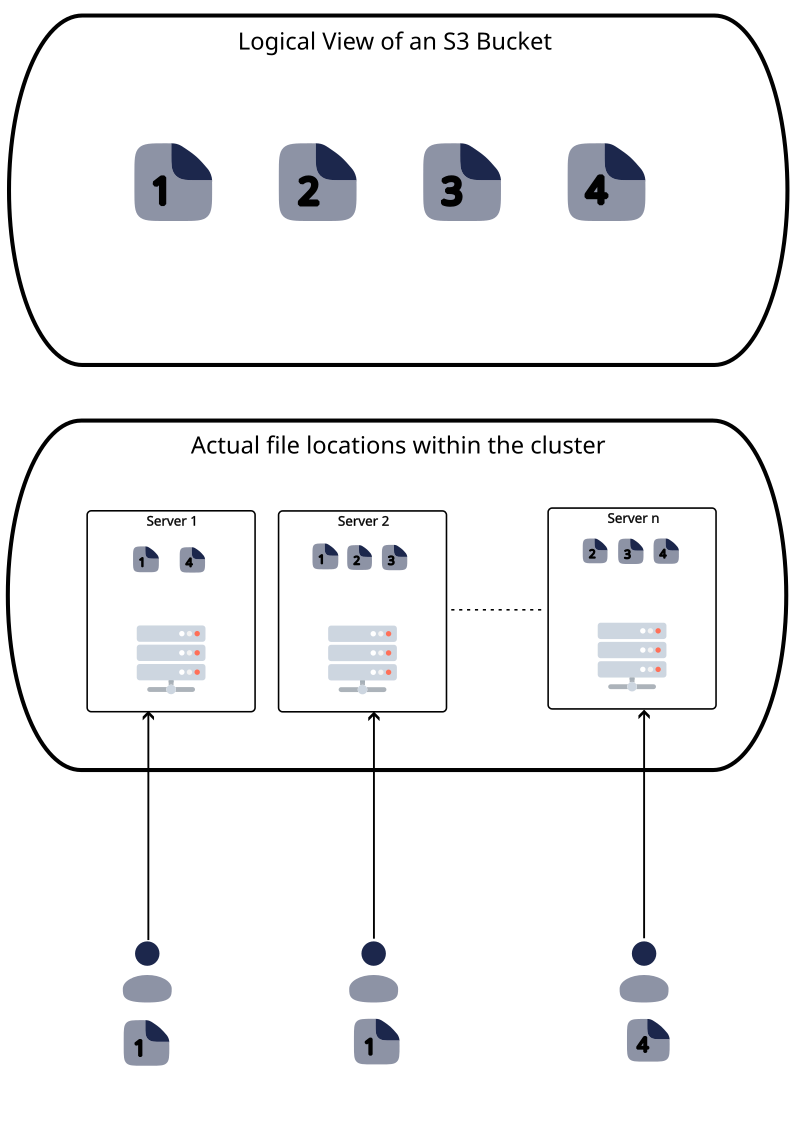
\includegraphics[width=0.6\textwidth]{figures/distributedCloudStorage.png}
    \caption{Distributed File Store}
    \label{fig:distFileStore}
\end{figure}

\medskip
The exact architecture of AWS S3 or any similar service provided by
competing cloud providers is not known, however, we can glean some information
about S3 based on
how other distributed filesystems were designed. We will explain some basic ideas
related to AWS S3 using Figure-\ref{fig:distFileStore}. Let us assume we need to
store four files in AWS S3. In order to do that, we first create a storage unit
called a `bucket' which is similar to a directory in a filesystem. After
uploading our files to this bucket, the files get replicated over the entire AWS S3 cluster in
that particular region. Figure-\ref{fig:distFileStore} assumes that this cluster
has a replication factor of two and therefore every file is stored on two
physical servers. Now, if users send requests to access these files, their
requests can be redirected to any one of the servers containing the desired file. For
example, if the first and second user both want to access file number 1, their
requests can be served by two different servers since the same copy will be
saved on two different servers. For simplicity, the figure shows that users make
direct requests to the physical machines containing these files, however, in
reality they all send requests to a single endpoint and their requests are then
redirected to a server based on some load balancing scheme. In later chapters,
we will use this abstract model of a distributed filesystem to argue about the
applicability of various techniques.

\medskip
Apart from the basic understanding of AWS S3 as it related to a distributed
filesystem, we also want to draw the reader's attention to the following
characteristics of AWS S3 as mentioned in its documentation:
\begin{enumerate}
    \item \textbf{Throughput SLA}: At the time of writing this paper, AWS
        gaurantees that S3 can handle at least 5500 requests per object stored
        in a bucket. Note that there is no restriction on the total number of
        objects that can be stored in a bucket.
    \item \textbf{Storage Classes}: S3 offers various storage classes that have
        different cost and performance characteristics. These storage classes
        determine how much you pay for storage and for making requests. In this
        thesis, we make use of the `S3 Standard' and `Express One Zone' storage
        classes.
    \item \textbf{Costs}: The cost of using AWS S3 depends on two factors: total
        storage and number of requests. The storage cost for `S3 Standard'
        storage class is \$0.023/GB and the cost of GET requests is
        \$0.0004/1k requests. However, the storage cost for the lower latency
        `Express One Zone' storage type is higher with \$0.16/GB but the cost of making
        requests is lower at \$0.0002/1k requests. 
    \item \textbf{Artificial subdirectories}: Although AWS CLI and other tools
        provide the capability to upload and navigate a bucket like a directory,
        but the underlying architecture only supports having files inside a
        bucket. Therefore, if you have a folder `f1' with two files `one' and
        `two', unlike a filesystem, the bucket would only contain two files
        namely: `f1/one' and `f1/two'. The name of the folder is simply
        prepended to the file names.
    \item \textbf{Hashing object names}: In order to decide which partitions an
        object is assigned to, S3 internally hashes the first few characters of
        the filename. Therefore, if we have object names whose first few
        characters are the same, it is possible they will all be assigned to a
        single partition which may lead to lower performance. Although, it is
        mentioned that S3 automatically splits partitions in case of overload,
        there is some overhead and time delay in performing the split.
\end{enumerate}

\section{Serverless Database Architectures}\label{sec:serverlessArch}
The term `serverless' was originally used in relation to peer to peer
communication where a server is not required to communicate between two
machines. However, since the advent of cloud computing, this term has been
commandeered by cloud providers to mean something entirely different. In the
context of cloud computing, the term `serverless computing' is the culmination 
of a trend of
separating application logic from the underlying hardware resources. This trend
began with the advent of virtual machines, was carried forward by
containerization technologies like Docker, and culminated in serverless services
like AWS Lambda. At every step along the way, the developers lost some control
over the hardware and in return got increased development velocity and reduced
infrastructure maintainance overhead.

% Write about serverless databases.
\medskip
Serverless Databases.

 

\section{Caching and Prefetching in distributed systems}\label{sec:cachingDistSys}
